\section{Notation and Definitions}
\label{app:notation}

\begin{table}[H]
\centering
\scriptsize
\renewcommand{\arraystretch}{0.90}
\begin{tabular}{p{3.0cm}p{9.8cm}}
\toprule
Symbol & Meaning in the Interpreter Model \\
\midrule
$\varphi_Q$ & Timeless relational field, represented in the formal model by the relational sector of the global quantum state and used as the shared server basis. \\
$B_i$ & Locally stored life history and the resulting individual configuration of interpreter $i$. \\
$B_i(t)$ & Current bodily, adaptive, and attentional configuration of the local interpreter. \\
$I_{\mathrm{syn}}(t)$ & Current locally available sensory and bodily input. \\
$D_i^{\mathrm{local}}$ & Complete local side: $B_i$, $B_i(t)$, $I_{\mathrm{syn}}(t)$, and the physical client configuration. \\
$\Gamma_{\mathrm{server}}$ & Timeless network extracted from the correlation effects of the global relational state. \\
$\Gamma_i^{(n)}$ & Weighted projection of $\Gamma_{\mathrm{server}}$ produced by interpreter $i$ during mapping cycle $n$. \\
$\mathcal J_i^{(\leq n)}$ & Realised relations encountered up to event $n$ in the local causal order of interpreter $i$. \\
$\hat C_\gamma$ & Positive effect representing relation $\gamma$ in the relational sector, with $0\leq\hat C_\gamma\leq I$. \\
$\Pi_i^{(n)}$ & Local conditioning projector fixed by interpreter $i$'s causal address and event index. \\
$\omega_{i\gamma}^{(n)}$ & Effective weight of server relation $\gamma$ in interpreter $i$'s current mapping cycle. \\
$e_{i\gamma}^{(n)},m_{i\gamma}^{(n)}$ & Conditionally available relation strength and its local mappability factor. \\
$a_{i\gamma}^{\mathrm{bio}},\mu_{i\gamma}$ & Biographical affinity and pattern overlap used in local weighting. \\
$\operatorname{dist}_{h_i}(p_i,p_\gamma),|\Delta s_{i\gamma}|$ & Invariant distance on the local rest slice and local proper-time separation from relation $\gamma$. \\
$H_i$ & Biological hardware presently available to interpreter $i$. \\
$D_i^{\mathrm{server},(n)}$ & Conditionally available server-side relation data $(\gamma,e_{i\gamma}^{(n)})$ passed to mapping cycle $n$ before local mappability and weighting are applied. \\
$\mathfrak B_i^{(n)}$ & Relation-indexed carrier branches that are both available in cycle $n$ and physically realisable by the current biological hardware. \\
$u_i^\mu$ & Future-directed local timelike vector $dx_i^\mu/ds_i$ that orders mapped relations along interpreter $i$'s physical worldline; $s_i$ is local proper time. \\
$h_{\mu\nu}^{(i)}$ & Induced spatial metric on the local rest slice $\Sigma_i$ orthogonal to $u_i^\mu$. \\
$K_i$ & One bidirectional conditioning, comparison, spacetime mapping, physical realisation, rendering, and inscription process. \\
$E_G,e_G$ & Total Penrose gravitational self-energy difference of two Orch-OR branch mass profiles, and the corresponding single-dimer contribution used in the geometric scaling calculation. \\
$\sigma_\nu,\Delta R$ & Width of nuclear Gaussian profile $\nu$ and displacement between its two branch positions. \\
$\tau_i$ & Locally measured collapse interval of one rendering event. \\
$w_i(t)$ & Adaptive neuronal current that carries recent firing history and changes the effective local trigger. \\
$q_{ik}(s)$ & Occupation of the lowest collective vibrational mode in candidate carrier domain $k$. \\
$n_{ik},\Omega_i(s),N_i(s)$ & Dimer population of domain $k$, set of recruited domains, and total recruited dimer count $\sum_{k\in\Omega_i(s)}n_{ik}$ at local time $s$. \\
$A_i(s)$ & Accumulated dimensionless Orch-OR action $\hbar^{-1}\int_0^sE_G(s')ds'$. \\
$N_i^*$ & Total recruited dimer count immediately before the endogenous Orch-OR threshold is reached. \\
$N_G^*(\tau_i)$ & Stationary carrier count obtained from the independently evaluated geometric $E_G$. \\
$N_{\mathrm{HP}}^*(\tau_i)$ & Literature-anchored carrier count for interval $\tau_i$ in the additive Hameroff--Penrose benchmark. \\
$\Psi_i$ & Experiential image formed during $K_i$; the mapping event itself is conscious. \\
$G_i$ & Data gap detected in the local state after a mapping disruption. \\
$C_i$ & Maximum weighted convergence of a relational pattern in the current mapping cycle. \\
$\mathcal F_i$ & Fidelity of source, perspective, event detail, and temporal assignment; $\mathcal F_{i,\mathrm{event}}$ denotes event-detail fidelity. \\
$T_{i,\mathrm{resp}}$ & Measured interval from cue onset to a stable response in the prospective relational-convergence test. \\
\bottomrule
\end{tabular}
\caption{Notation used throughout the paper.}
\label{tab:notation}
\end{table}

\section{Neurodynamic and Biological Implementation}
\label{app:neurodynamic}

\subsection{Carrier constraints and source values}

\begin{table}[H]
\centering
\footnotesize
\begin{tabular}{@{}
  >{\raggedright\arraybackslash}p{3.0cm}
  >{\raggedright\arraybackslash}p{5.2cm}
  >{\raggedright\arraybackslash}p{5.0cm}@{}}
\toprule
Source & System or intervention & Result used here \\
\midrule
\citet{frohlich1968} & metabolically driven polar structures & collective vibrational modes \\
\citet{zhang2019frohlich,wang2022frohlich} & driven molecular vibrations & pump threshold, gain--loss dynamics, and nonequilibrium phase transition \\
\citet{preto2026} & driven classical protein-mode Hamiltonian in a 300 K bath & Fr\"ohlich-type condensation across common coupling rescaling from $0.01$ to $1$; bath-mediated low-frequency nonlinear coupling required \\
\citet{engel2007} & photosynthetic complex (FMO) at 77 K & long-lived electronic coherence in energy transfer \\
\citet{panitchayangkoon2010,collini2010} & photosynthetic complexes at physiological and ambient temperature & warm biological coherence \\
\citet{ishiwata2026} & pentacene molecular spins in nanocrystals inside living cells & intracellular Rabi control and spin echo; $T_2\sim1\,\mu\mathrm{s}$ and $T_1\sim75\,\mu\mathrm{s}$ \\
\citet{babcock2024} & tryptophan networks and tubulin assemblies & ultraviolet superradiant modes and enhanced quantum yield \\
\citet{mavromatos2025} & ordered-water/microtubule QED cavity & estimated decoherence interval $10^{-7}$--$10^{-6}$ s \\
\citet{craddock2017} & collective tubulin-mode model & anaesthetic-dependent mode change \\
\citet{kalra2023} & purified microtubules; isoflurane and etomidate & $D=(3.15\pm0.10)\times10^{-5}\,\mathrm{cm^2\,s^{-1}}$; $L=6.64\pm0.10$ nm; reduced transport \\
\citet{khan2024} & epothilone~B arm, eight male rats (12 animals in the study); 0.75 mg/kg; 4 percent isoflurane & loss of righting reflex delayed 69 s; permutation $t$-test $p=0.0016$; $d=1.9$ \\
\citet{li2025} & prolonged microtubule-modulating drug treatment in mice & drug-specific shifts in isoflurane sensitivity, induction, and emergence \\
\citet{huang2026} & mice; one 8 mg/kg epothilone~B dose & following-day delay 29 s; $d=0.8$ \\
\bottomrule
\end{tabular}
\caption{Theoretical, experimental, and intervention results used in the biological
carrier account.}
\label{tab:biological_carrier_constraints}
\end{table}

\subsection{Macroscopic neural field}

The neural population follows a one-population Wilson--Cowan reduction
\citep{wilsoncowan1972}.
\begin{equation}
  \tau_E \frac{\partial E(\mathbf{x},t)}{\partial t}
  = -E(\mathbf{x},t)
  + \mathcal S\left[
      \int W_E(\mathbf{x}-\mathbf{x}')E(\mathbf{x}',t)\,d^3x'
      + P(\mathbf{x},t)
    \right].
  \label{eq:wilsoncowan}
\end{equation}
\noindent Here $E$ is the population activity, $\tau_E$ the population time
constant, $W_E$ the spatial kernel, and $\mathcal S$ a dimensionally normalised
sigmoid. $P$ is the local sensory, bodily, and realised-carrier drive.

\subsection{Adaptive single neuron}

The single neuron follows the Adaptive Exponential Integrate-and-Fire reduction
\citep{hodgkinhuxley1952,brettegerstner2005}.
\begin{align}
  C_m \frac{dV}{dt} &=
    -g_L(V-E_L)
    + g_L\Delta_T\exp\left(\frac{V-V_T}{\Delta_T}\right)
    - w_i + I_{\mathrm{ext}},
  \label{eq:adex_V}\\
  \tau_w \frac{dw_i}{dt} &= a(V-E_L)-w_i.
  \label{eq:adex_w}
\end{align}
\noindent At each spike the neuron is reset by $V\leftarrow V_r$ and
$w_i\leftarrow w_i+b$. With $w_i$ held fixed, the exponential term places the
subthreshold saddle at $V=V_T$. This gives the effective trigger current
\begin{equation}
  I_{\theta,i}^{\mathrm{eff}}(t)
  \simeq g_L(V_T-E_L-\Delta_T)+w_i(t).
  \label{eq:adaptive_trigger}
\end{equation}
\noindent The time $t$ is identified with the proper time $s_i$ on the local
worldline.

\section[Quantum-Gravitational Coupling and Derivations]
{Quantum-Gravitational Coupling\\and Derivations}
\label{app:quantum_coupling}

\subsection{Timeless state and server relations}

The starting point is the Wheeler--DeWitt constraint \citep{dewitt1967}.
\begin{equation}
  \hat H|\Phi\rangle=0,
  \qquad
  \hat H=\hat H_{\mathrm{grav}}+\hat H_{\mathrm{matter}}.
  \label{eq:wdw}
\end{equation}
Let $\rho_Q$ be the normalised state induced by $|\Phi\rangle$ on the relational
sector $\varphi_Q$. The server notation is the correlation map
\begin{equation}
  e_\gamma=\operatorname{Tr}(\rho_Q\hat C_\gamma),
  \qquad
  \Gamma_{\mathrm{server}}
  =\left\{\gamma:e_\gamma>0\right\},
  \qquad 0\leq\hat C_\gamma\leq I.
  \label{eq:server_relation_encoding}
\end{equation}
At the local address selected by $\Pi_i^{(n_i)}$, the relation strength passed to
$K_i$ is
\begin{equation}
  e_{i\gamma}^{(n_i)}=
  \frac{\operatorname{Tr}\!\left(
    \Pi_i^{(n_i)}\hat C_\gamma\Pi_i^{(n_i)}\rho_Q
  \right)}
  {\operatorname{Tr}\!\left(\Pi_i^{(n_i)}\rho_Q\right)},
  \qquad \operatorname{Tr}\!\left(\Pi_i^{(n_i)}\rho_Q\right)>0.
  \label{eq:server_relation_read}
\end{equation}
The complete server-side input to cycle $n_i$ is therefore
\begin{equation}
  D_i^{\mathrm{server},(n_i)}=
  \left\{(\gamma,e_{i\gamma}^{(n_i)}):
  \gamma\in\Gamma_{\mathrm{server}},\ e_{i\gamma}^{(n_i)}>0\right\}.
  \label{eq:available_server_data}
\end{equation}
It contains conditionally available relations and their read strengths. Local
mappability, effective weights, and the projection $\Gamma_i^{(n_i)}$ are formed
only after these data enter $K_i$.
The realised event changes the local configuration and local event history:
\begin{equation}
  B_i^{(n_i+1)}=B_i^{(n_i)}\oplus\Psi_i^{(n_i)},
  \qquad
  \mathcal J_i^{(\leq n_i+1)}
  =\mathcal J_i^{(\leq n_i)}\cup\{\gamma_i^{(n_i)}\},
  \qquad \gamma_i^{(n_i)}\in\Gamma_{\mathrm{server}}.
  \label{eq:server_relation_write}
\end{equation}
\noindent Here $\oplus$ denotes local incorporation, $\gamma_i^{(n_i)}$ the realised
relation, and $n_i$ the local causal event index. The global $\rho_Q$ and
$\Gamma_{\mathrm{server}}$ carry no $n_i$ evolution. Equation~\eqref{eq:server_relation_write}
is the internal read/write description of a relation in the ordered local history,
not evolution under an external server clock \citep{pagewootters1983}.

\subsection{CDT and the local time vector}

CDT sums over causal triangulations \citep{ambjorn2004}.
\begin{equation}
  Z_{\mathrm{CDT}}=
  \sum_{T\in\mathcal T_{\mathrm{causal}}}\frac{1}{C_T}
  \exp\!\left[-\frac{S_E[T]}{\hbar}\right].
  \label{eq:cdt}
\end{equation}
\noindent Here $C_T$ is the symmetry factor and $S_E[T]$ the Euclideanised
discretised action. Each $T\in\mathcal T_{\mathrm{causal}}$ is an admissible
foliation and gluing.

Only an effective continuum geometry is passed forward from the CDT ensemble.
\begin{equation}
  \left\{T\in\mathcal T_{\mathrm{causal}}\right\}_{Z_{\mathrm{CDT}}}
  \xrightarrow{\ \mathcal C_\ell\ }
  (\overline M,\overline g_{\mu\nu}^{(\ell)}),
  \qquad \ell\gg a_{\mathrm{CDT}}.
  \label{eq:cdt_coarse_geometry}
\end{equation}
\noindent Here $\mathcal C_\ell$ is the coarse-graining in a semiclassical CDT
sector, and $a_{\mathrm{CDT}}$ is the lattice scale
\citep{ambjorn2004,benedetti2007}.

On the resulting patch, the local tetrad and spin frame are normalised by
\begin{equation}
  \overline g_{\mu\nu}^{(\ell)}=
  e_{\mu}^{AA'}(\ell)e_{\nu}^{BB'}(\ell)\epsilon_{AB}\epsilon_{A'B'},
  \qquad
  \xi_{i,\ell}^{AA'}=e_{\mu}^{AA'}(\ell)\xi_i^\mu.
  \label{eq:cdt_spinframe}
\end{equation}
\noindent Here $\overline g_{\mu\nu}^{(\ell)}$ is the effective local Lorentzian
metric and $e_\mu^{AA'}$ the spin frame. $\xi_{i,\ell}^{AA'}$ is the bispinor form
of the Riemann-normal coordinate $\xi_i^\mu\in T_{p_i}\overline M$
\citep{speziale2012}.

The future-directed local tangent of the client's worldline is
\begin{equation}
  u_i^\mu=\frac{dx_i^\mu}{ds_i},
  \qquad
  \overline g_{\mu\nu}^{(\ell)}u_i^\mu u_i^\nu=-1
  \quad(c=1),
  \label{eq:local_time_vector}
\end{equation}
\noindent Here $s_i$ is the proper time and $\tau_i$ the local collapse interval. A
shared relation is weighted on each of the two worldlines,
$\gamma_{ij}\mapsto(\omega_{i\gamma_{ij}},\omega_{j\gamma_{ij}})$.

Within the normal neighbourhood of the local event, the same geometry defines the
spatial rest section used by the branch-density calculation:
\begin{equation}
  h_{\mu\nu}^{(i)}=
  \overline g_{\mu\nu}^{(\ell)}+u_{i\mu}u_{i\nu},
  \qquad
  h_{\mu\nu}^{(i)}u_i^\nu=0,
  \qquad
  d\mu_{h_i}=\sqrt{\det h_{mn}^{(i)}}\,d^3x .
  \label{eq:cdt_rest_slice}
\end{equation}
\noindent Here $h_{mn}^{(i)}$ is the positive spatial metric induced on the local
section $\Sigma_i$ orthogonal to $u_i$. Its Green kernel is fixed by
\begin{equation}
  -\Delta_{h_i}\mathcal G_{h_i}(x,y)=4\pi\delta_{h_i}(x,y),
  \qquad
  \mathcal G_{h_i}(x,y)
  \xrightarrow{\ \ell^2\|\operatorname{Riem}\|\ll1\ }
  \frac{1}{|\mathbf x-\mathbf y|}.
  \label{eq:cdt_green_kernel}
\end{equation}
\noindent The kernel is selected by decay at spatial infinity in the local
asymptotically flat limit, or by the corresponding Dirichlet boundary data when the
normal neighbourhood is represented by a finite computational patch.

\subsection{Twistor incidence as spacetime address}

Twistor incidence is used only in the flat tangent space at the local event, not as
a global twistor construction on the curved CDT geometry \citep{penrose1967,frauendiener2000}:
\begin{equation}
  \mathcal L_{\xi_i}^{\mathrm{loc}}=
  \left\{Z^\alpha=(\omega^A,\pi_{A'}):
  \omega^A=i\,\xi_{i,\ell}^{AA'}\pi_{A'}\right\},
  \qquad \ell^2\|\operatorname{Riem}(\overline g^{(\ell)})\|\ll1.
  \label{eq:twistor_incidence}
\end{equation}
\noindent Here $Z^\alpha=(\omega^A,\pi_{A'})$ is a twistor, and
$\mathcal L_{\xi_i}^{\mathrm{loc}}$ is the incidence set used as the local address. No
transport of one global twistor through an arbitrary curved spacetime is required.

\subsection{Weighted relational access in local spacetime}

The weighted domain depends on the cycle.
\begin{equation}
  \Gamma_i^{(n)}=
  \left\{\left(\gamma,\omega_{i\gamma}^{(n)}\right):
  (\gamma,e_{i\gamma}^{(n)})\in D_i^{\mathrm{server},(n)}\right\},
  \qquad 0\leq\omega_{i\gamma}^{(n)}\leq1.
  \label{eq:weighted_relational_domain}
\end{equation}
Each weight is the product of two factors.
\begin{align}
  \omega_{i\gamma}^{(n)}
    &=e_{i\gamma}^{(n)}\,m_{i\gamma}^{(n)},
    \label{eq:relation_weight}\\
  m_{i\gamma}^{(n)}
    &=\mathcal W_i\!\left(
      \operatorname{dist}_{h_i}(p_i,p_\gamma),|\Delta s_{i\gamma}^{(n)}|,
      a_{i\gamma}^{\mathrm{bio}},
      \mu_{i\gamma},G_i^{(n)};
      B_i,B_i(t),I_{\mathrm{syn}}(t),H_i
    \right).
    \label{eq:relation_mappability}
\end{align}
\noindent Here $e_{i\gamma}^{(n)}$ is the conditionally available relation strength
from Eq.~\eqref{eq:server_relation_read}, $a_{i\gamma}^{\mathrm{bio}}$ the
biographical affinity, $\mu_{i\gamma}$ the pattern overlap, and $H_i$ the available
hardware. $\operatorname{dist}_{h_i}(p_i,p_\gamma)$ is the invariant spatial distance
between the local event and the relation address on the rest slice of $u_i$, and
$|\Delta s_{i\gamma}|$ is the local proper-time separation. The model
restricts $0\leq e_{i\gamma}^{(n)},m_{i\gamma}^{(n)}\leq1$ and requires $\mathcal W_i$
to depend on local geometric invariants rather than coordinate labels. Holding the
other inputs fixed,
\begin{equation}
  \frac{\partial m_{i\gamma}}{\partial a_{i\gamma}^{\mathrm{bio}}}\geq0,
  \qquad
  \frac{\partial m_{i\gamma}}{\partial \mu_{i\gamma}}\geq0,
  \qquad
  \frac{\partial m_{i\gamma}}{\partial |\Delta s_{i\gamma}|}\leq0,
  \qquad
  \frac{\partial m_{i\gamma}}
              {\partial\operatorname{dist}_{h_i}(p_i,p_\gamma)}\leq0.
  \label{eq:mappability_constraints}
\end{equation}
These bounds constrain one shared weighting rule across applications.

\subsection{One conditioning and mapping process}

Within $K_i$, weighted branch formation gives the pre-reduction state
\begin{equation}
  |\chi_i^{(n_i)}(0)\rangle
  =\sum_{(\gamma,a)\in\mathfrak B_i^{(n_i)}}
    c_{i,\gamma,a}^{(n_i)}|\chi_{i,\gamma,a}\rangle.
  \label{eq:conditioned_branch_state}
\end{equation}
The realisable branch set is
\begin{equation}
  \mathfrak B_i^{(n)}=
  \left\{(\gamma,a):
  (\gamma,\omega_{i\gamma}^{(n)})\in\Gamma_i^{(n)},\ 
  |\chi_{i,\gamma,a}\rangle\in
  \mathcal H_i^{\mathrm{phys}}[B_i(t),H_i]\right\}.
  \label{eq:realisable_branch_set}
\end{equation}
\noindent Here $a$ indexes the alternative carrier branches associated with an
available relation $\gamma$.
The positive normaliser and the weighted coefficients are
\begin{equation}
\begin{aligned}
  \mathcal Z_i^{(n)}
    &=\sum_{(\delta,b)\in\mathfrak B_i^{(n)}}
      \omega_{i\delta}^{(n)}
      \left|\widetilde c_{i,\delta,b}^{(n)}\right|^2>0,\\
  c_{i,\gamma,a}^{(n)}
    &=\frac{\sqrt{\omega_{i\gamma}^{(n)}}\,
      \widetilde c_{i,\gamma,a}^{(n)}}
      {\sqrt{\mathcal Z_i^{(n)}}},\\
  \left|c_{i,\gamma,a}^{(n)}\right|^2
    &=\frac{\omega_{i\gamma}^{(n)}
      \left|\widetilde c_{i,\gamma,a}^{(n)}\right|^2}
      {\mathcal Z_i^{(n)}},\\
  \sum_{(\gamma,a)\in\mathfrak B_i^{(n)}}
    \left|c_{i,\gamma,a}^{(n)}\right|^2&=1.
\end{aligned}
  \label{eq:weighted_branch_coefficients}
\end{equation}
\noindent Here $\widetilde c_{i,\gamma,a}^{(n)}$ is the unweighted local carrier
amplitude, and $\rho_{i,\gamma,a}(x,s)$ is the branch mass density on the local rest
slice.

\paragraph{Consistency lemma (conditioning, Born probabilities, and no-signalling).}
Let the branch vectors in $\mathfrak B_i^{(n)}$ be orthonormal and let
$|\widetilde\chi_i\rangle=\sum_{(\gamma,a)}
\widetilde c_{i,\gamma,a}|\chi_{i,\gamma,a}\rangle$ have unit norm. Define
\begin{equation}
  L_i=\sum_{(\gamma,a)\in\mathfrak B_i^{(n)}}
    \sqrt{\omega_{i\gamma}^{(n)}}\,
    |\chi_{i,\gamma,a}\rangle\langle\chi_{i,\gamma,a}|,
  \qquad
  \overline L_i=\left(I-L_i^\dagger L_i\right)^{1/2}.
  \label{eq:weighted_filter_instrument}
\end{equation}
Because $0\leq\omega_{i\gamma}^{(n)}\leq1$,
$L_i^\dagger L_i+\overline L_i^\dagger\overline L_i=I$. The maps generated by
$L_{i,1}=L_i$ and $L_{i,0}=\overline L_i$ therefore form a completely positive
two-outcome instrument, with non-selective channel
\begin{equation}
  \mathcal E_i(\rho)=\sum_{r=0}^{1}L_{i,r}\rho L_{i,r}^\dagger,
  \qquad
  \sum_{r=0}^{1}L_{i,r}^\dagger L_{i,r}=I.
  \label{eq:weighted_filter_channel}
\end{equation}
Conditioning on $r=1$ gives Eq.~\eqref{eq:weighted_branch_coefficients} exactly.
The ordinary Born rule is then applied to this prepared state; $\omega$ is not a
second probability rule. For uniform nonzero weights,
\begin{equation}
  \omega_{i\gamma}^{(n)}=\omega_0>0\quad\text{for every }(\gamma,a)
  \quad\Longrightarrow\quad
  c_{i,\gamma,a}^{(n)}=\widetilde c_{i,\gamma,a}^{(n)},
  \label{eq:weighted_standard_limit}
\end{equation}
so the unweighted prepared state is recovered. At $\omega_0=1$,
\begin{equation}
  L_i=P_{\mathfrak B_i^{(n)}},
  \qquad
  L_i|\widetilde\chi_i\rangle=|\widetilde\chi_i\rangle,
  \label{eq:weighted_unit_projector}
\end{equation}
where $P_{\mathfrak B_i^{(n)}}$ is the projector on the prepared branch space. The
instrument $\mathcal E_i$ acts on the local carrier Hilbert space
$\mathcal H_i^{\mathrm{phys}}$; no completeness of $\mathfrak B_i^{(n)}$ in that full
space is assumed.

For a joint state $\rho_{ij}$ and any trace-preserving operation
$\Lambda_j^{(\alpha_j)}$ selected with free setting $\alpha_j$ at a spacelike separated event
$p_j$, require the locally incident weights and $\mathcal E_i$ to be independent of
$\alpha_j$. The local-address rule enforces this until $p_j$ lies in the causal past of
the mapped event $p_i$:
\begin{equation}
  p_j\notin J^-(p_i)
  \quad\Longrightarrow\quad
  \frac{\partial\Pi_i^{(n)}}{\partial \alpha_j}=0,
  \qquad
  \frac{\partial\omega_{i\gamma}^{(n)}}{\partial \alpha_j}=0.
  \label{eq:local_setting_independence}
\end{equation}
Then
\begin{equation}
  \operatorname{Tr}_j\!\left[
    (\mathcal E_i\otimes\Lambda_j^{(\alpha_j)})(\rho_{ij})
  \right]
  =\mathcal E_i\!\left(\operatorname{Tr}_j\rho_{ij}\right),
  \label{eq:weighted_filter_no_signalling}
\end{equation}
which is independent of $\alpha_j$. Existing server relations may correlate conditioned
outcomes, but neither client can choose the local outcome or change the other's
non-selective marginal. This is the density-matrix no-signalling condition
\citep{simon2001nosignaling}.

\subsection{Operational individuality}

Let $X$ collect one admissible common relation/input condition and every component of
the canonical input tuple in Eq.~\eqref{eq:core_model} except the locally stored
configuration. Using the same mapping functional $K$ on both inputs, operational
distinguishability is
\begin{equation}
  B_i\not\equiv_K B_j
  \quad\Longleftrightarrow\quad
  \exists X:\ K[X;B_i]\not\equiv K[X;B_j].
  \label{eq:individuality}
\end{equation}
This requires one distinguishing condition, not a different mapped content for
every difference between two biological configurations. The neural state evolution
is already specified by AdEx and Wilson--Cowan, so no additional automaton dynamics
is introduced here.

For one shared relation pattern $\mathcal R_j\subset\Gamma_{\mathrm{server}}$,
different local configurations enter two complete mapping cycles:
\begin{equation}
  \Psi_i=K_i\!\left[D_i^{\mathrm{local}}(B_i),
    D_i^{\mathrm{server}}(\mathcal R_j),G_i\mid u_i\right],
  \\
  \Psi_k=K_k\!\left[D_k^{\mathrm{local}}(B_k),
    D_k^{\mathrm{server}}(\mathcal R_j),G_k\mid u_k\right].
  \label{eq:shared_relation_local_mappings}
\end{equation}

\subsection{Pre-reduction quantum-potential form guidance}

Let $\mathbf X=(\mathbf x_1,\ldots,\mathbf x_{N_{\mathrm{dof}}})$ collect the coordinates of the
carrier constituents in the local rest frame, with masses $m_\alpha$, and write
$\psi_i(\mathbf X,s_i)=R_i(\mathbf X,s_i)e^{iS_i(\mathbf X,s_i)/\hbar}$ with $R_i>0$
\citep{bohm1952a}. The configuration-space quantum potential is
\begin{equation}
  Q_i[R_i]=-\frac{1}{R_i}
    \sum_{\alpha=1}^{N_{\mathrm{dof}}}\frac{\hbar^2}{2m_\alpha}\nabla_\alpha^2R_i,
  \qquad Q_i[cR_i]=Q_i[R_i]\quad(c>0).
  \label{eq:bohm_Q}
\end{equation}
In the local rest frame, phase and amplitude evolve by
\begin{equation}
  \frac{\partial S_i}{\partial s_i}
  +\sum_{\alpha=1}^{N_{\mathrm{dof}}}\frac{|\nabla_\alpha S_i|^2}{2m_\alpha}
  +V_i+Q_i[R_i]=0,
  \qquad
  \frac{\partial R_i^2}{\partial s_i}
  +\sum_{\alpha=1}^{N_{\mathrm{dof}}}\nabla_\alpha\!\cdot\!\left(
    R_i^2\frac{\nabla_\alpha S_i}{m_\alpha}\right)=0.
  \label{eq:bohm_local_guidance}
\end{equation}
\noindent These equations have a pre-reduction role only. Eqs.~\eqref{eq:bohm_Q}
and~\eqref{eq:bohm_local_guidance} evolve
$|\chi_i(0)\rangle\rightarrow|\chi_i(s_i)\rangle$, and $Q$ neither selects nor
reweights an $\omega$-weighted branch. No definite Bohmian beable trajectory is
introduced.
The scale-invariant quantum-potential term carries form before reduction, Orch~OR
fixes the state, and biological terms power and amplify the carrier.

\subsection{Recruited mass-density branches and objective reduction}

For the recruited carrier-domain set $\Omega_i(s)$, let $\mathcal D_{ik}$ be the
tubulin dimers in domain $k$ and $n_{ik}=|\mathcal D_{ik}|$. Fix relation $\gamma$
and suppress that index during the mass-density calculation. The regularised branch
density on the CDT-induced local rest slice is
\begin{equation}
  \rho_{i,a}(x,s)=
  \sum_{k\in\Omega_i(s)}\sum_{d\in\mathcal D_{ik}}
  \sum_{\nu\in\mathcal N_d}
  m_\nu f_{\sigma_\nu}^{(h_i)}(x,x^{a}_{kd\nu}),
  \qquad
  \int_{\Sigma_i}f_{\sigma_\nu}^{(h_i)}(x,x^{a}_{kd\nu})\,d\mu_{h_i}(x)=1,
  \label{eq:branch_density}
\end{equation}
\noindent Here $k$ is a recruited carrier domain, $d$ a tubulin dimer, and $\nu$ a
massive constituent. $f_{\sigma_\nu}$ is the normalised profile of width
$\sigma_\nu$. For the same fixed $\gamma$, the branch difference is
$\Delta\rho_{ab}=\rho_{i,a}-\rho_{i,b}$, and the branch displacement is
$\mathbf x^a_{kd\nu}-\mathbf x^b_{kd\nu}$.

The local weak-field Penrose gravitational self-energy functional is
\begin{equation}
  E_G^{ab}(s;h_i)=
  \frac{G}{2}
  \int_{\Sigma_i}d\mu_{h_i}(x)
  \int_{\Sigma_i}d\mu_{h_i}(y)\,
  \Delta\rho_{ab}(x,s)\mathcal G_{h_i}(x,y)\Delta\rho_{ab}(y,s).
  \label{eq:eg}
\end{equation}
\noindent $E_G$ has the unit joule, $[E_G]=\mathrm J$.
Equations~\eqref{eq:cdt_green_kernel}
and~\eqref{eq:eg} recover the Newtonian $1/|\mathbf x-\mathbf y|$ expression in the
local flat limit. The full density retains self and cross terms, so its scaling is
computed from the recruited geometry rather than assigned as $N$ or $N^2$
\citep{hameroff2014,figurato2024,tomaz2024}.

The numerical calculation uses normalised Gaussian nuclear profiles. Their exact
pair kernel in the local flat limit is
\begin{equation}
  f_{\sigma_\nu}(\mathbf x)=
  \frac{e^{-|\mathbf x|^2/(2\sigma_\nu^2)}}{(2\pi\sigma_\nu^2)^{3/2}},
  \qquad
  \mathcal U_{\nu\mu}(R)=
  \begin{cases}
    \displaystyle
    \frac{\operatorname{erf}\!\left(
      R/\sqrt{2(\sigma_\nu^2+\sigma_\mu^2)}
    \right)}{R}, & R>0,\\[1.0ex]
    \displaystyle
    \frac{\sqrt{2/\pi}}{\sqrt{\sigma_\nu^2+\sigma_\mu^2}}, & R=0.
  \end{cases}
  \label{eq:gaussian_mass_kernel}
\end{equation}
For two discrete branch geometries this gives
\begin{equation}
  E_G^{ab}=\frac{G}{2}\sum_{\alpha,\beta}m_\alpha m_\beta
  \left[
    \mathcal U_{\alpha\beta}(R_{\alpha\beta}^{aa})
    +\mathcal U_{\alpha\beta}(R_{\alpha\beta}^{bb})
    -\mathcal U_{\alpha\beta}(R_{\alpha\beta}^{ab})
    -\mathcal U_{\alpha\beta}(R_{\alpha\beta}^{ba})
  \right].
  \label{eq:geometric_eg_discrete}
\end{equation}
The self terms are evaluated exactly. For distinct nuclei or dimers,
$\Delta R\ll R_{\alpha\beta}$ permits the stable expansion
\begin{equation}
  E_{G,\alpha\beta}^{\mathrm{cross}}
  =-Gm_\alpha m_\beta\,
  \mathbf d_\alpha^{\mathsf T}
  \nabla\nabla\!\left(\frac{1}{R_{\alpha\beta}}\right)
  \mathbf d_\beta
  +O\!\left(\frac{Gm_\alpha m_\beta\Delta R^3}{R_{\alpha\beta}^4}\right).
  \label{eq:geometric_cross_expansion}
\end{equation}
For a common rigid displacement the odd orders cancel and the displayed remainder
begins at $O(Gm_\alpha m_\beta\Delta R^4/R_{\alpha\beta}^5)$.

The Orch-OR action condition is \citep{penrose1996,hameroff2014}
\begin{equation}
  \int_0^{\tau_i}E_G(s)\,ds\sim\hbar,
  \qquad
  E_G(s)=E_G\ \Longrightarrow\
  \tau_i\sim\frac{\hbar}{E_G}.
  \label{eq:or_time}
\end{equation}
\noindent The numerical order-one factor is set to unity. The two-state ratio is
given in Eq.~\eqref{eq:or_ratio_test}. In this construction $E_G$ fixes the reduction
threshold and its time. Outcome probabilities remain the ordinary Born probabilities
of the conditioned state in Eq.~\eqref{eq:weighted_branch_coefficients}. Diósi's
separate stochastic completion of the same $E_G/\hbar$ rate introduces a universal
noise term and correlation length $R_0$ \citep{diosi2022}; neither enters this cycle.

\subsection{Recruitment and Orch-OR threshold}

Let $q_{ik}=\langle n_{0,ik}\rangle$ be the lowest-mode occupation of candidate
carrier domain $k$. The mean-field gain--loss terms derived for a driven
Fr{\"o}hlich mode are \citep{zhang2019frohlich,wang2022frohlich}
\begin{equation}
\begin{aligned}
  r_{ik}^{\mathrm{eff}}(s)
    &=r_{ik}[B_i,w_i(s),I_{\mathrm{syn}}(s)]
      +\sum_{l\sim k}J_{kl}\bigl(q_{il}(s)-q_{ik}(s)\bigr),\\
  N_{r,ik}(s)
    &=\frac{(D_{ik}^{\mathrm{mode}}+1)r_{ik}^{\mathrm{eff}}(s)}{\phi_{ik}},\\
  \mathcal P_{ik}(s)
    &=N_{r,ik}(s)+(D_{ik}^{\mathrm{mode}}+1)\bar n_{ik},\\
  g_{ik}(s)
    &=\kappa_{ik}N_{r,ik}(s)-\phi_{ik}-\kappa_{ik},\\
  \frac{dq_{ik}}{ds}
    &=g_{ik}q_{ik}-\kappa_{ik}q_{ik}^{2}
      +r_{ik}^{\mathrm{eff}}+\phi_{ik}\bar n_{ik}
      +\kappa_{ik}(\bar n_{ik}+1)\mathcal P_{ik}.
\end{aligned}
  \label{eq:coupled_frohlich_recruitment}
\end{equation}
\noindent The last line uses the published mean-field closure
$\langle n_{0,ik}^2\rangle\simeq q_{ik}^2$. Here $D_{ik}^{\mathrm{mode}}$ is the
number of coupled vibrational modes, $\phi_{ik}$ the loss rate, $\kappa_{ik}$ the
nonlinear redistribution rate, and $\mathcal P_{ik}$ the total phonon population.
$J_{kl}=J_{lk}\geq0$ is the symmetric carrier coupling. Admissible states have
$r_{ik}^{\mathrm{eff}}\geq0$. The network term sums to zero and
therefore preserves the total supplied pump rate,
$\sum_k r_{ik}^{\mathrm{eff}}=\sum_k r_{ik}$. It redistributes the biological drive
among coupled domains but does not provide another energy source. The onset threshold
is
\begin{equation}
  r_{c,ik}=\frac{\phi_{ik}}{D_{ik}^{\mathrm{mode}}+1}
  \left(1+\frac{\phi_{ik}}{\kappa_{ik}}\right),
  \qquad
  g_{ik}>0\ \Longleftrightarrow\ r_{ik}^{\mathrm{eff}}>r_{c,ik}.
  \label{eq:frohlich_recruitment_threshold}
\end{equation}
The neighbour term allows one condensed domain to recruit another. It supplies the
network-cascade mechanism without identifying cascade size with gravitational
self-energy \citep{diazpalencia2025}. The use of $g_{ik}>0$ below is a binary onset
approximation: a domain contributes its structurally specified dimer population once
its linear gain becomes positive. It introduces no additional fitted threshold.
Before reduction,
\begin{equation}
  \Omega_i(s)=\{k:g_{ik}(s)>0\},
  \qquad N_i(s)=\sum_{k\in\Omega_i(s)}n_{ik}.
  \label{eq:coherent_domain}
\end{equation}

Recruitment and reduction are coupled by
\begin{equation}
\begin{aligned}
  A_i(s)&=\frac{1}{\hbar}\int_0^s
  E_G[\Delta\rho_i(s');h_i]\,ds',\\
  \tau_i&=\inf\{s>0:A_i(s)\geq1\},
  \qquad
  N_i^*=\lim_{s\uparrow\tau_i}N_i(s).
\end{aligned}
  \label{eq:adaptive_or_trigger}
\end{equation}
\noindent Equation~\eqref{eq:frohlich_recruitment_threshold} starts collective
recruitment. Equation~\eqref{eq:adaptive_or_trigger} terminates its coherent
pre-reduction development. The stationary limit is $E_G\tau=\hbar$. The neuronal
state variable is given in Eq.~\eqref{eq:adaptive_trigger}.

\subsection{Geometric mass-density evaluation}

The independent calculation uses the heavy-nucleus coordinates of the 1JFF
alpha--beta tubulin structure \citep{lowe2001}. It contains 6,578 modelled heavy
atoms in 838 of 896 deposited residues. The missing residue fraction is restored
once as a factor of $896/838$. A 13-protofilament cylinder with an 8 nm axial dimer
spacing supplies the recruited domain geometry \citep{fourniol2010}. Neither a
collapse interval nor a per-dimer gravitational energy is used as a calibration.

The 2.5 fm carbon-profile input has two common Gaussian readings. Treating it as
the radius of a uniform sphere gives $\sigma_C=a_C/\sqrt{5}$; treating it directly
as the Gaussian width gives $\sigma_C=a_C$. Table~\ref{tab:geometric_eg_profiles}
shows the sensitivity to this choice. For a nucleus of mass number $A_\nu$, the
calculation uses
\begin{equation}
  \sigma_\nu=\sigma_C\left(\frac{A_\nu}{12}\right)^{1/3}.
  \label{eq:nuclear_profile_scaling}
\end{equation}
Relative to assigning the carbon width to every nucleus, this profile rule lowers
$e_G(2.5\,\mathrm{fm})$ by 10.03 percent in the sphere-equivalent reading and
11.45 percent in the direct-width reading.

\begin{table}[H]
\centering
\scriptsize
\resizebox{\textwidth}{!}{%
\begin{tabular}{@{}lrrrrrrrrr@{}}
\toprule
& \multicolumn{5}{c}{Finite-profile saturation}
& \multicolumn{4}{c}{Carrier counts $N_G^*$} \\
\cmidrule(lr){2-6}\cmidrule(l){7-10}
Profile reading & $\sigma_C$ [fm] & $e_G(\infty)$ [J/dimer]
& $e_G(2.5)/e_G(\infty)$ & $\Delta R_{50}$ [fm] & $\Delta R_{90}$ [fm]
& $500$ ms; $2.5$ fm & $25$ ms; $2.5$ fm
& $500$ ms; $\infty$ & $25$ ms; $\infty$ \\
\midrule
Sphere-equivalent Gaussian & 1.118 & $1.125\times10^{-43}$ & 0.280 & 4.088 & 20.750
& $6.688\times10^9$ & $1.338\times10^{11}$ & $1.875\times10^9$ & $3.749\times10^{10}$ \\
Direct Gaussian width & 2.500 & $5.031\times10^{-44}$ & 0.0718 & 9.140 & 46.399
& $5.839\times10^{10}$ & $1.168\times10^{12}$ & $4.192\times10^9$ & $8.384\times10^{10}$ \\
\bottomrule
\end{tabular}%
}
\caption{Finite-profile saturation from Eq.~\eqref{eq:geometric_eg_discrete} and
stationary carrier counts $N_G^*=\hbar/(\tau e_G)$. The two rows bracket the
profile-width interpretation without fitting the result to an Orch-OR interval; the
$\infty$ columns give the smallest counts available from each finite profile.}
\label{tab:geometric_eg_profiles}
\end{table}

\noindent These are total recruited dimer counts. They may be distributed across
carrier domains and are not the length of one 13-protofilament cylinder.

For comparison, the published additive Hameroff--Penrose anchors satisfy
\begin{equation}
\begin{aligned}
  N\tau&\simeq5.0\times10^8\ \mathrm{tubulin\,s},
  &\epsilon_{G,\mathrm{HP}}&=2.11\times10^{-43}\ \mathrm{J\,tubulin^{-1}},\\
  N_{\mathrm{HP}}^*(\tau_i)
  &=N_{500}\frac{500\ \mathrm{ms}}{\tau_i},
  \qquad N_{500}=10^9.
\end{aligned}
  \label{eq:hp_anchor_scaling}
\end{equation}

\begin{table}[H]
\centering
\footnotesize
\begin{tabular}{@{}rrrrp{4.0cm}@{}}
\toprule
$\tau_i$ & $E_G$ [J] & $N_{\mathrm{HP}}^*$ & $N_{\mathrm{HP}}^*/10^9$ & Role \\
\midrule
25 ms  & $4.218\times10^{-33}$ & $2.000\times10^{10}$ & 20.000 & Orch-OR 40 Hz reference \\
500 ms & $2.109\times10^{-34}$ & $1.000\times10^9$  & 1.000  & Orch-OR 500 ms reference \\
\bottomrule
\end{tabular}
\caption{Published anchors of the historical additive scenario
\citep{hameroff2014}. Table~\ref{tab:geometric_eg_profiles} contains the operative
calculation.}
\label{tab:historical_hp_anchors}
\end{table}

\begin{figure}[H]
  \centering
  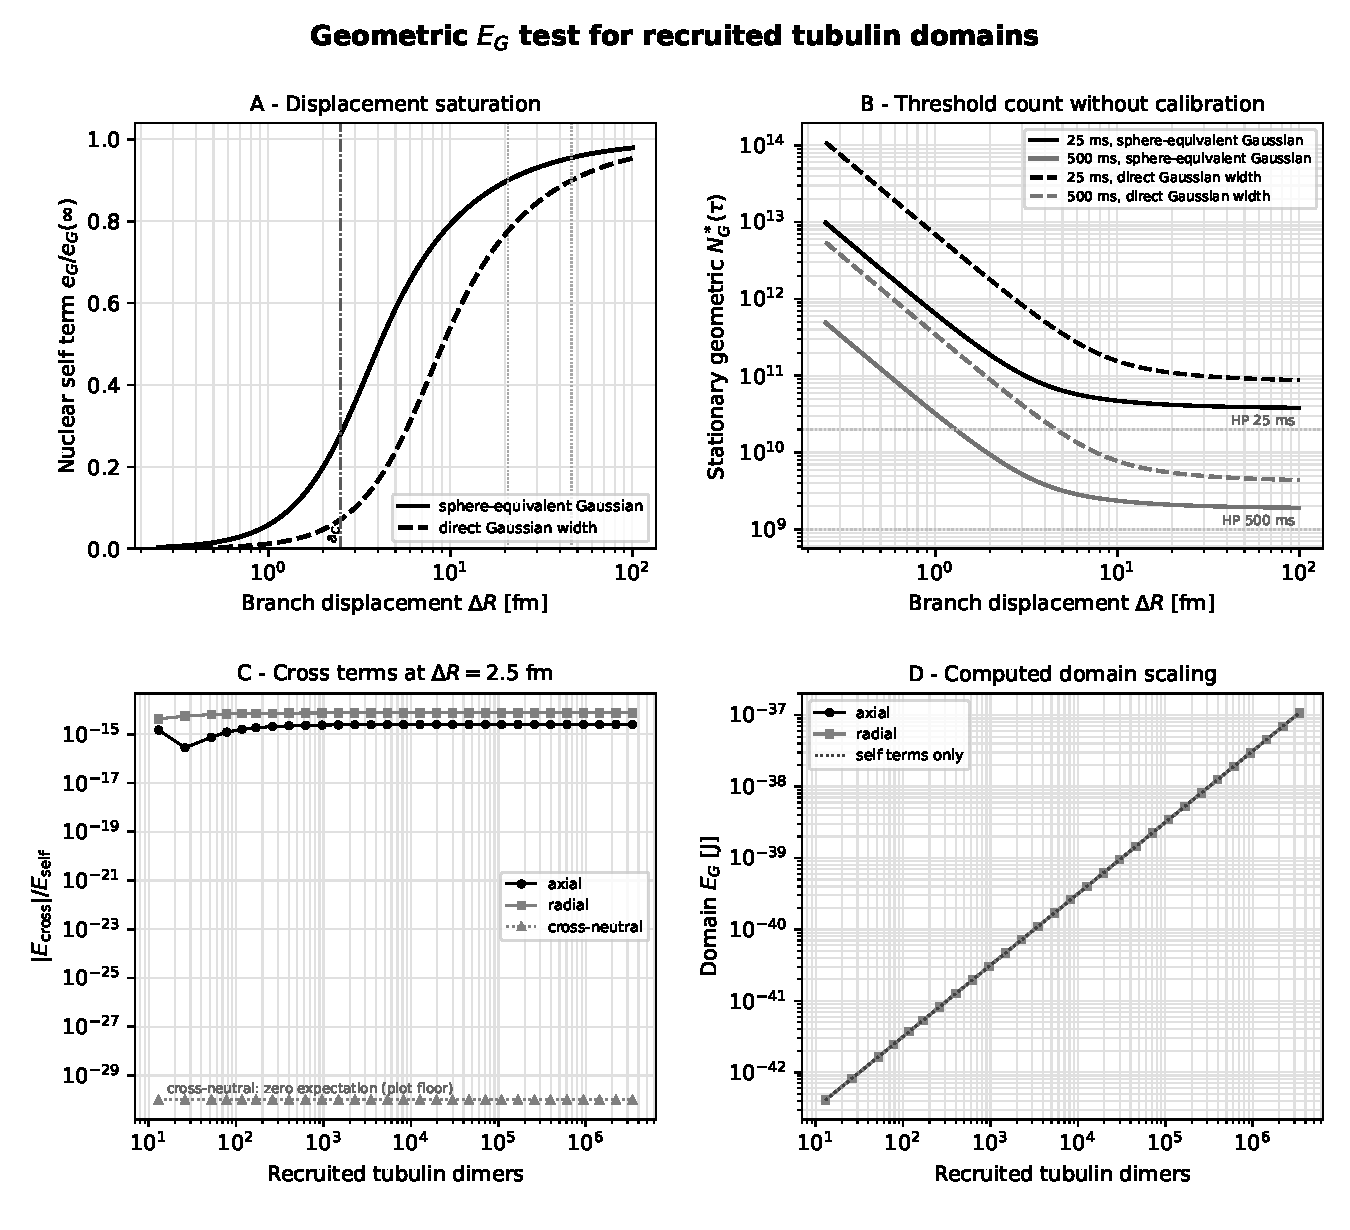
\includegraphics[width=0.94\textwidth]{data/geometric_eg_sweep.pdf}
  \caption{Finite-profile saturation, uncalibrated threshold counts, retained cross
  terms, and domain scaling. At 3,407,872 dimers the axial and radial cross fractions
  are $-2.507\times10^{-15}$ and $+7.535\times10^{-15}$.}
  \label{fig:geometric_eg_sweep}
\end{figure}

\begin{samepage}
\paragraph{Recruitment--reduction lemma.}
For the distributed rigid-displacement geometries evaluated here, write the
single-dimer self term as $e_G(\Delta R,\sigma)$ and the complete domain energy as
\begin{equation}
  E_G(s)=e_G(\Delta R,\sigma)N_i(s)[1+\delta_i(s)],
  \qquad |\delta_i(s)|\leq\varepsilon_{\mathrm{geom}}<1.
  \label{eq:recruitment_reduction_linearisation}
\end{equation}
The numerical sweep gives $\varepsilon_{\mathrm{geom}}<7.6\times10^{-15}$ through
3,407,872 dimers for the tested axial and radial orientations. The pair-Hessian bound
$|\mathbf d_\alpha^{\mathsf T}\nabla\nabla(1/r)\mathbf d_\beta|
\leq2\Delta R^2/r^3$ gives the per-dimer axial lattice remainder beyond $L$ layers:
\begin{equation}
  \left|e_{\mathrm{cross}}^{(\infty)}-e_{\mathrm{cross}}^{(L)}\right|
  \leq
  \frac{2P\,Gm_d^2\Delta R^2}{a_z^3L^2},
  \label{eq:geometric_cross_tail_bound}
\end{equation}
where $P=13$, $a_z=8$ nm, and $m_d=101.93$ kDa. At $L=262144$ and
$\Delta R=2.5$ fm, the bound is $8.84\times10^{-69}$ J per dimer, or
$2.81\times10^{-25}$ of the nuclear self term. For this finite-cross-section
geometry, the lattice contribution therefore has a convergent per-dimer limit and
cannot develop an $N^2$ term as cylinder length increases. The threshold tables give
the total count across recruited domains; cross-domain terms for any specified
arrangement remain governed by Eq.~\eqref{eq:eg} rather than by an assumed scaling
rule. Substitution into
Eq.~\eqref{eq:adaptive_or_trigger} gives
\begin{equation}
  \frac{\hbar}{e_G(1+\varepsilon_{\mathrm{geom}})}
  \leq \int_0^{\tau_i}N_i(s)\,ds
  \leq \frac{\hbar}{e_G(1-\varepsilon_{\mathrm{geom}})},
  \qquad
  \overline N_i=\frac{1}{\tau_i}\int_0^{\tau_i}N_i(s)\,ds.
  \label{eq:recruitment_reduction_bound}
\end{equation}
Reduction therefore depends on accumulated recruitment rather than an
instantaneous carrier count. Different pump trajectories reach the same threshold
when they supply the same integrated load within these geometric bounds.
\end{samepage}

\begin{table}[H]
\centering
\scriptsize
\renewcommand{\arraystretch}{0.88}
\begin{tabular}{@{}
  >{\raggedright\arraybackslash}p{3.2cm}
  >{\raggedright\arraybackslash}p{4.0cm}
  >{\raggedright\arraybackslash}p{5.2cm}@{}}
\toprule
Input & Value and status & Use in the calculation \\
\midrule
Nuclear profile & $a_C\simeq2.5$ fm; few-fm branch displacement; literature model choice \citep{hameroff2014} & Finite branch-density profile in $E_G$; not identified with a stochastic noise length $R_0$. \\
Tubulin geometry & 1JFF alpha--beta dimer; 6,578 modelled heavy atoms and 838/896 deposited residues \citep{lowe2001} & Supplies the independent nuclear coordinates and the completeness correction. \\
Domain geometry & 13 protofilaments, 8 nm axial dimer spacing \citep{fourniol2010} & Supplies the distributed recruitment lattice for the cross-term and domain-size sweep. \\
Profile-width sweep & $\sigma_C=a_C/\sqrt{5}$ and $\sigma_C=a_C$; $\sigma_\nu=\sigma_C(A_\nu/12)^{1/3}$ & Brackets two readings of the 2.5 fm profile input and records the mass-number scaling used for non-carbon nuclei. \\
Electronic separation & order 1 nm; literature model choice \citep{hameroff2014} & Physical route associated by Orch OR with the nuclear-scale displacement. \\
Carrier anchor & $10^9$ tubulins at 500 ms and $2\times10^{10}$ at 25 ms; approximate literature result \citep{hameroff2014} & Fixes $\epsilon_{G,\mathrm{HP}}$ and the conditional $N_{\mathrm{HP}}^*(\tau_i)$ benchmark. \\
Recruitment law & Pump, loss, redistribution, and network coupling \citep{zhang2019frohlich,wang2022frohlich,diazpalencia2025} & Determines $\Omega_i(s)$ and $N_i(s)$ before reduction. \\
Geometric scaling & Full molecular and lattice mass-density calculations \citep{figurato2024,tomaz2024}; Table~\ref{tab:geometric_eg_profiles} & Evaluates self and cross terms on the CDT-induced rest geometry. \\
\bottomrule
\end{tabular}
\caption{Parameter provenance for the geometric $E_G$ and recruitment calculation.}
\label{tab:orch_or_parameter_provenance}
\end{table}

\noindent\begin{minipage}{\linewidth}
\noindent\textit{Stochastic-model comparison.}
LISA Pathfinder gives $\sigma_{\mathrm{DP}}>(40.1\pm0.5)$ fm; Gran Sasso excludes
the natural Markovian version; XENONnT gives $R_0>4.5\times10^{-10}$ m at 95\% CL
\citep{helou2017,donadi2021,xenon2026collapse}. These bounds apply to universal DP
noise dynamics. Their noise lengths are not inputs to the Orch-OR branch calculation.
\end{minipage}

All steps compose into one dependency chain.
\begin{equation}
  \begin{gathered}
  \begin{aligned}
  \hat H|\Phi\rangle=0
  &\longmapsto \rho_Q
  \xrightarrow{\ \operatorname{Tr}(\rho_Q\hat C_\gamma)\ }
  \Gamma_{\mathrm{server}},\\
  \{T\}_{Z_{\mathrm{CDT}}}
  &\xrightarrow{\ \mathcal C_\ell\ }
  (\overline g_{\mu\nu}^{(\ell)},e_\mu^{AA'},u_i^\mu,
   h_{\mu\nu}^{(i)},\mathcal G_{h_i})
  \longmapsto \mathcal L_{\xi_i}^{\mathrm{loc}},\\
  (\Gamma_{\mathrm{server}},\mathcal L_{\xi_i}^{\mathrm{loc}},n)
  &\xrightarrow{\ \Pi_i^{(n)},\ \mathrm{Eq.}\,\eqref{eq:server_relation_read}\ }
  D_i^{\mathrm{server},(n)}.
  \end{aligned}\\[-2pt]
  \underbrace{\begin{aligned}
  (D_i^{\mathrm{local}},D_i^{\mathrm{server}},G_i;u_i)
  &\longmapsto \Gamma_i^{(n)}(\omega_{i\gamma}^{(n)})
  \longmapsto \mathfrak B_i^{(n)}
  \longmapsto |\chi_i(0)\rangle,\\
  |\chi_i(0)\rangle
  &\xrightarrow[\ s_i<\tau_i\ ]{\ Q,\ r^{\mathrm{eff}}/r_c\ }
  (|\chi_i(s_i)\rangle,\Omega_i(s_i),N_i(s_i)),\\
  (|\chi_i(s_i)\rangle,\Omega_i(s_i))
  &\xrightarrow{\ \Delta\rho_i[h_i],\ E_G,\ A_i(\tau_i)=1\ }
  |\chi_i^{\mathrm{fixed}}\rangle,\\
  |\chi_i^{\mathrm{fixed}}\rangle
  &\xrightarrow{\ \mathrm{AdEx/Wilson--Cowan}\ }\Psi_i,\\
  \Psi_i
  &\xrightarrow{\ \mathrm{Eq.}\,\eqref{eq:server_relation_write}\ }
  (B_i^{(n+1)},\mathcal J_i^{(\leq n+1)};
   \gamma_i^{(n)}\in\Gamma_{\mathrm{server}}),\\
  (B_i^{(n+1)},\mathcal J_i^{(\leq n+1)};
   \gamma_i^{(n)}\in\Gamma_{\mathrm{server}})
  &\rightsquigarrow K_i^{(n+1)}\text{ input conditions}.
  \end{aligned}}_{K_i^{(n)}\text{: one conscious mapping cycle}}
  \end{gathered}
  \label{eq:physical_chain}
\end{equation}
\section{Model Tests and Numerical Results}
\label{app:model_tests}

\subsection{Finite local associative load}

With the load $\alpha=P/N$ and the critical value $\alpha_c\simeq0.14$
\citep{amit1985}, the critical number of patterns is
\begin{equation}
  P_{\mathrm{crit}}\simeq\alpha_c N\simeq0.14N.
  \label{eq:hopfield_finite_load}
\end{equation}
\noindent A finite number of units gives a finite critical load,
$N<\infty\Rightarrow P_{\mathrm{crit}}<\infty$.

\subsection{Measured relational convergence}

Let
\begin{equation}
  \operatorname{Rel}\!\left(\Gamma_i^{(n)}\right)=
  \left\{\gamma:(\gamma,\omega_{i\gamma}^{(n)})\in\Gamma_i^{(n)},\ 
  \omega_{i\gamma}^{(n)}>0\right\}
  \label{eq:available_relation_support}
\end{equation}
be the relation support available in the current cycle. For
$\mathcal R_j\subseteq\operatorname{Rel}(\Gamma_i^{(n)})$ and normalisable cycle
weights, define
\begin{equation}
  d_{ij}^{(n)}=
  \frac{\displaystyle\sum_{\gamma\in\mathcal R_j}\omega_{i\gamma}^{(n)}}
       {\displaystyle\sum_{\gamma\in\operatorname{Rel}(\Gamma_i^{(n)})}
         \omega_{i\gamma}^{(n)}}.
  \label{eq:relational_dominance}
\end{equation}
For at least two nonzero-weight relations, let $r_{\gamma\delta}\in[0,1]$ denote
their model-level semantic or causal relation strength. Then
\begin{equation}
  \eta_{ij}^{(n)}=
  \frac{\displaystyle
    \sum_{\substack{\gamma,\delta\in\mathcal R_j\\\gamma\neq\delta}}
      r_{\gamma\delta}\,
      \omega_{i\gamma}^{(n)}\omega_{i\delta}^{(n)}}
       {\displaystyle
    \sum_{\substack{\gamma,\delta\in\mathcal R_j\\\gamma\neq\delta}}
      \omega_{i\gamma}^{(n)}\omega_{i\delta}^{(n)}}.
  \label{eq:relational_coherence}
\end{equation}
Convergence is
\begin{equation}
  C_{ij}^{(n)}=d_{ij}^{(n)}\eta_{ij}^{(n)},
  \qquad
  C_i^{(n)}=\max_j C_{ij}^{(n)}.
  \label{eq:weighted_convergence}
\end{equation}
The definitions give $0\leq d_{ij}^{(n)},\eta_{ij}^{(n)},C_{ij}^{(n)},C_i^{(n)}\leq1$.

The measured centrality of event $\gamma$ is \citep{leechen2022}
\begin{equation}
  r_\gamma=
  \operatorname{Norm}_{\mathrm{narrative}}\!\left(
    \sum_{\delta\neq\gamma}s_{\gamma\delta}
  \right),
  \label{eq:measured_relational_centrality}
\end{equation}
\noindent$s_{\gamma\delta}$ is the measured semantic similarity or independently
judged causal relation used to estimate the model quantity $r_{\gamma\delta}$.

\begin{table}[H]
\centering
\footnotesize
\begin{tabular}{@{}
  >{\raggedright\arraybackslash}p{3.0cm}
  >{\raggedright\arraybackslash}p{5.5cm}
  >{\raggedright\arraybackslash}p{4.2cm}@{}}
\toprule
Source and sample & Measured comparison & Result used here \\
\midrule
\citet{horner2015}, $N=26$ & closed-loop dependency against independent retrieval & $t(25)=2.57$, $p<0.05$; derived $d_z=0.504$ \\
\citet{horner2015}, $N=26$ & open-loop dependency against independent retrieval & $t(25)=1.80$, $p=0.08$; derived $d_z=0.353$ \\
\citet{horner2015}, $N=26$ & closed-loop--open-loop dependency difference & $t(25)=2.77$, $p<0.05$; derived $d_z=0.543$ \\
\citet{horner2015}, $N=26$ & incidental non-target reinstatement & $t(25)=3.40$, $p<0.01$; derived $d_z=0.667$ \\
\citet{leechen2022}, $N=393$ & unique semantic and causal centrality effects on recall & $\beta=0.17$ and $0.44$, both $p<0.001$; logistic mixed models, $\chi^2$ tests \\
\citet{leechen2022}, $N=15$ & high--low centrality hippocampal recall activity & $t(14)=2.71$, $p=0.017$, $d_z=0.70$ \\
\citet{leechen2022}, $N=15$ & high--low semantic-centrality PMC convergence during recall & $\Delta\mathrm{pISC}=0.019$, $p=0.037$; randomisation test \\
\bottomrule
\end{tabular}
\caption{Source-derived relational-convergence benchmark. Horner et al. isolate
network closure at equal relation count; Lee and Chen measure centrality, recall, and
cross-participant neural convergence. The $d_z$ values for Horner et al. are the
direct transformation $t/\sqrt{N}$. Lee and Chen's raw data are archived at
\href{https://doi.org/10.18112/openneuro.ds004042.v1.0.0}{OpenNeuro ds004042}; their
behavioural data and annotations are archived at
\href{https://github.com/jchenlab-jhu/filmfest}{jchenlab-jhu/filmfest}.}
\label{tab:relational_convergence_data}
\end{table}

Because relation structure is measured before recall, this benchmark requires no
model calibration. The prospective comparison and its recorded variables are given in
Table~\ref{tab:relational_convergence_protocol}.

\begin{table}[H]
\centering
\footnotesize
\begin{tabular}{@{}p{3.0cm}p{4.8cm}p{5.3cm}@{}}
\toprule
Protocol element & Specification & Recorded variables \\
\midrule
Shared condition & shared event anchor; complementary person, place, or object relations encoded in one local configuration & isolated retrieval from the other interpreter using the anchor as partial cue \\
Matched condition & same target; no shared event relation & identical retrieval procedure \\
Pre-registration & condition, target, correct response & fixed before measurement \\
Outcomes & forced choice and response process & accuracy, response time, confidence stability, incidental non-target reconstruction, source/perspective errors \\
\bottomrule
\end{tabular}
\caption{Prospective relational-convergence protocol.}
\label{tab:relational_convergence_protocol}
\end{table}

With $B_i(t)$, $H_i$, $G_i$, cue exposure, target, task, and response method matched,
let $j_{\mathrm{target}}$ denote the preregistered target relation set and let
$T_{i,\mathrm{resp}}$ be the measured interval from cue onset to a stable response.
The prospective group-level hypothesis is
\begin{equation}
\begin{aligned}
  \mathbb{E}[C_{i,j_{\mathrm{target}}}\mid\mathrm{shared}]&>
    \mathbb{E}[C_{i,j_{\mathrm{target}}}\mid\mathrm{matched}],\\
  \mathbb{E}[\mathcal F_{i,\mathrm{event}}\mid\mathrm{shared}]&>
    \mathbb{E}[\mathcal F_{i,\mathrm{event}}\mid\mathrm{matched}],\\
  \mathbb{E}[T_{i,\mathrm{resp}}\mid\mathrm{shared}]&<
    \mathbb{E}[T_{i,\mathrm{resp}}\mid\mathrm{matched}].
\end{aligned}
  \label{eq:cross_client_convergence_hypothesis}
\end{equation}
\subsection{Adaptive trigger sensitivity}

For constant input, $w_i=a(V-E_L)$, and the saddle-node rheobase is
\begin{align}
  V_{\mathrm{rheo}}
    &=V_T+\Delta_T\ln\!\left(\frac{g_L+a}{g_L}\right),\\
  I_{\mathrm{rheo}}
    &=(g_L+a)\left[V_T-E_L
      +\Delta_T\ln\!\left(\frac{g_L+a}{g_L}\right)-\Delta_T\right].
  \label{eq:adex_rheobase}
\end{align}
Adaptation is tested over the complete displayed $I/I_{\mathrm{rheo}}$ domain. The two
initial states and numerical controls are given in
Table~\ref{tab:adaptive_trigger_provenance}; their first-spike latencies are shown in
Figure~\ref{fig:adaptive_trigger_sensitivity}.

\begin{table}[H]
\centering
\footnotesize
\begin{tabular}{@{}
  >{\raggedright\arraybackslash}p{3.0cm}
  >{\raggedright\arraybackslash}p{4.0cm}
  >{\raggedright\arraybackslash}p{5.7cm}@{}}
\toprule
Quantity & Value & Status and role \\
\midrule
$C_m,g_L,E_L,$\newline $V_T,\Delta_T$ & 281 pF, 30 nS, $-70.6$ mV, $-50.4$ mV, 2 mV & regular-spiking AdEx source parameters \citep{brettegerstner2005} \\
$\tau_w,a,b$ & 144 ms, 4 nS, 80.5 pA & source parameters defining adaptation \citep{brettegerstner2005} \\
$I_{\mathrm{rheo}}$ & 627.311 pA & derived from Eq.~\eqref{eq:adex_rheobase} \\
$I/I_{\mathrm{rheo}}$ & complete displayed sweep & unknown drive retained as a dimensionless independent variable \\
Integration step & 0.05 ms; checked at 0.025 ms & numerical control; maximum latency change 0.1 ms \\
\bottomrule
\end{tabular}
\caption{Parameter provenance for the adaptive-trigger calculation.}
\label{tab:adaptive_trigger_provenance}
\end{table}

\begin{figure}[ht]
  \centering
  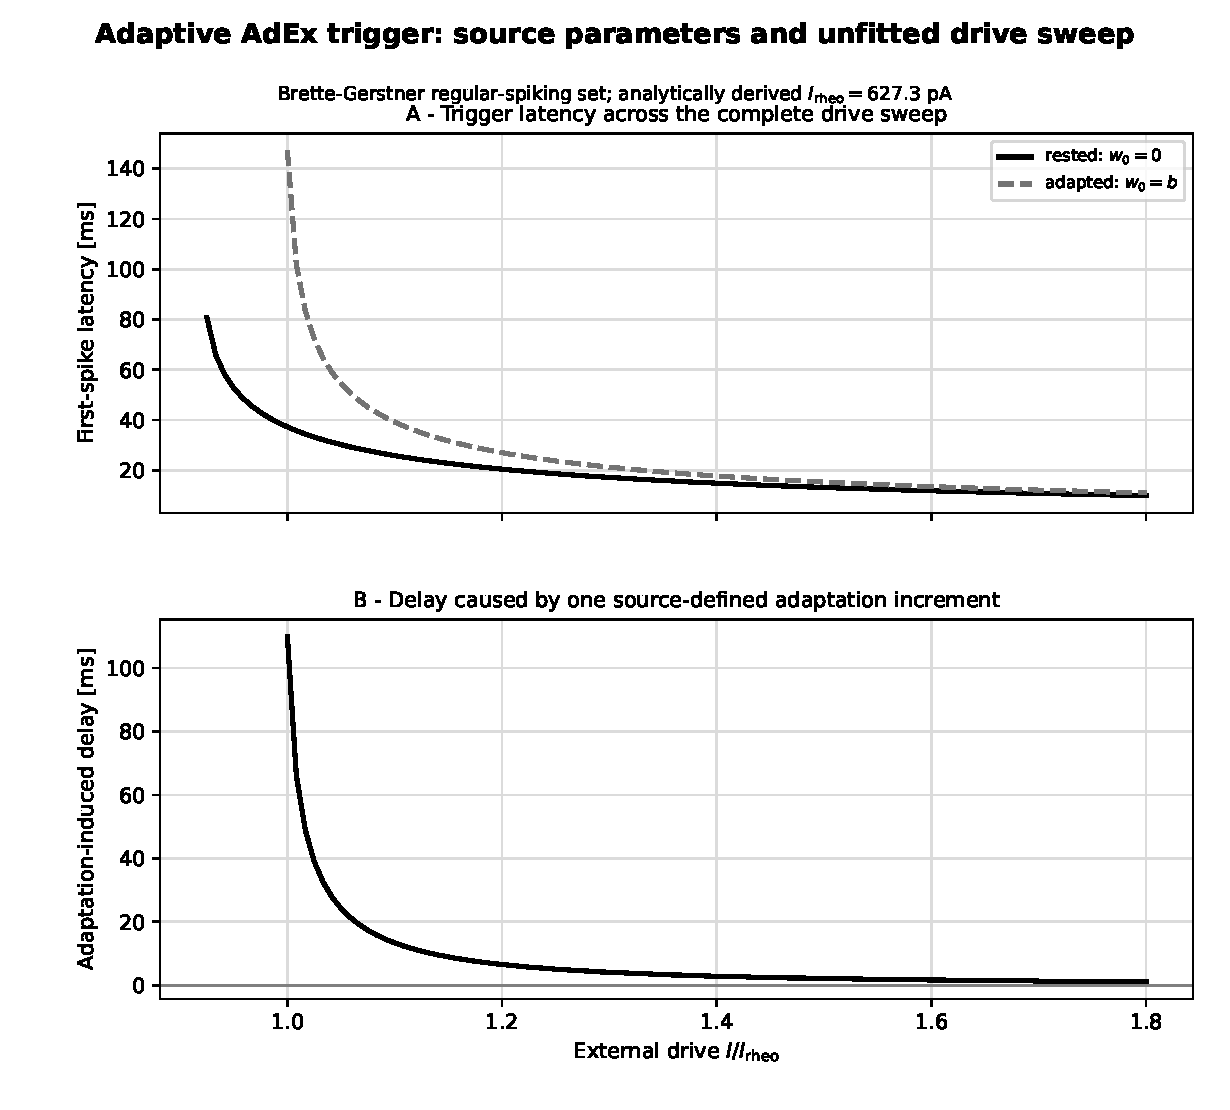
\includegraphics[width=\textwidth]{data/adaptive_trigger_sensitivity.pdf}
  \caption{AdEx trigger sensitivity. The source-defined adaptation increment changes
  first-spike latency across the source-parameterised drive sweep.}
  \label{fig:adaptive_trigger_sensitivity}
\end{figure}

\section{Mapping Disruption and Resynchronisation}
\label{app:mapping_disruption}

The gap is taken between the last stable local state at $t_0^-$ and the first
recovered state at $t_1^+$.
\begin{equation}
  G_i=\operatorname{Gap}\!\left(
    D_i^{\mathrm{local}}(t_0^-),D_i^{\mathrm{local}}(t_1^+)
  \right).
  \label{eq:mapping_gap}
\end{equation}
Resynchronisation repeats the complete mapping cycle.
\begin{align}
  \Psi_i^{(n)}
    &=K_i\!\left(
        D_i^{\mathrm{local},(n)},D_i^{\mathrm{server},(n)},G_i^{(n)}
        \mid u_i
      \right),
      \label{eq:resynchronisation_map}\\
  G_i^{(n+1)}&\subseteq G_i^{(n)},
  \qquad
  G_i^{(n+1)}=\varnothing
  \quad\text{when resynchronisation completes}.
  \label{eq:residual_mapping_gap}
\end{align}
\noindent Here $G_i^{(n+1)}$ is the unresolved remainder passed to the next cycle,
and $\mathcal F_i$ is the fidelity of source, perspective, event, and time.
Inscription follows Eqs.~\eqref{eq:physical_chain}
and~\eqref{eq:server_relation_write}.
